\chapter{Stand-alone heuristics}
On this chapter we will illustrate some stand-alone heuristics. These algorithms are so called because they provide an heuristic solution without relying on CPLEX or any other solver. The literature in this case is huge: there are plenty of different approaches and each of them can have multiple variations. On this report we will cover some of the major ideas. \\
For all the experiments to collect data for the performance profiles and the comparison between different algorithms we used a dataset of 20 instances, with a size between 400 and 3000 points. A detailed list of all the instances used and their dimension can be found on the tables of the section 5.4.

\section{Heuristic solution builder}
On this section we will illustrate some heuristics algorithm to generate in a rapid way a solution for the TSP problem. Of course the results provided by these algorithms are admissible solutions but not the optimum solution.

\subsection{Nearest neighborhood}
Nearest neighborhood is a greedy algorithm \footnote{algorithm that always makes the choice that looks best at the moment. That is, it makes a locally optimal choice in the hope that this choice
will lead to a globally optimal solution \cite{10.5555/1614191}.	 
} that works in the following way: start from a random point that is considered the first visited node. Then pick as next node the nearest to the last visited (greedy choice) and iterate until all the nodes are visited. This procedure can be repeated until a time limit is reached, each time starting from a different random point, keeping in memory the best solution and eventually update it if a new one is found. The algorithm is pretty simple but provide an admissible solution (that of course is not the best one and in the very most of the cases is quite far from the optimum) in a short time. \\

\begin{figure}[h!]
  \centering
  \begin{subfigure}[b]{0.49\linewidth}
    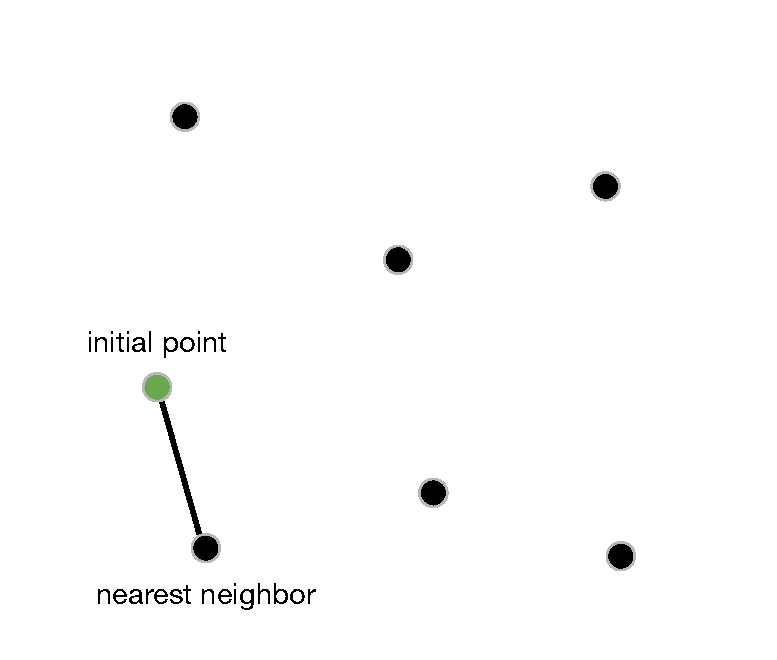
\includegraphics[width=\linewidth]{media/fase1.pdf}
     \caption{Initial step}
  \end{subfigure}
  \begin{subfigure}[b]{0.49\linewidth}
    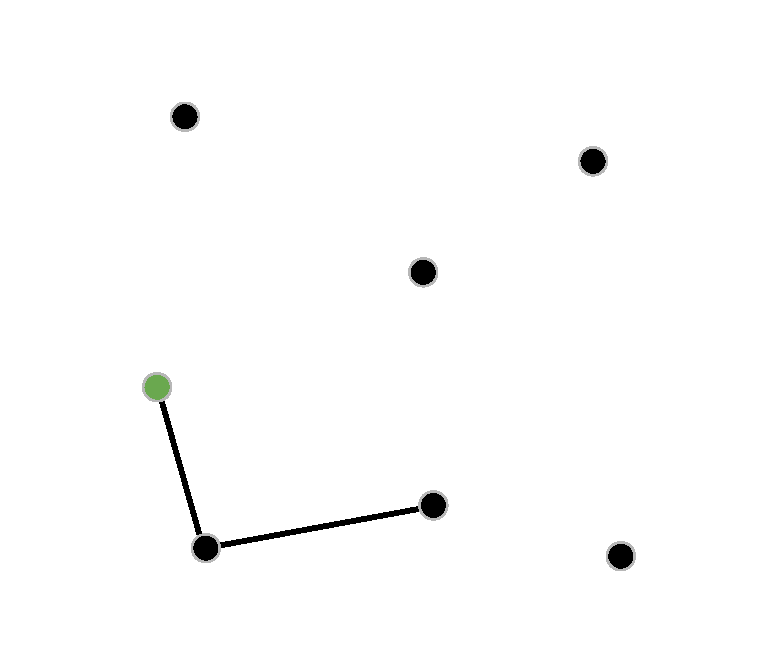
\includegraphics[width=\linewidth]{media/fase2.pdf}
    \caption{Second step}
  \end{subfigure}
  \begin{subfigure}[b]{0.49\linewidth}
    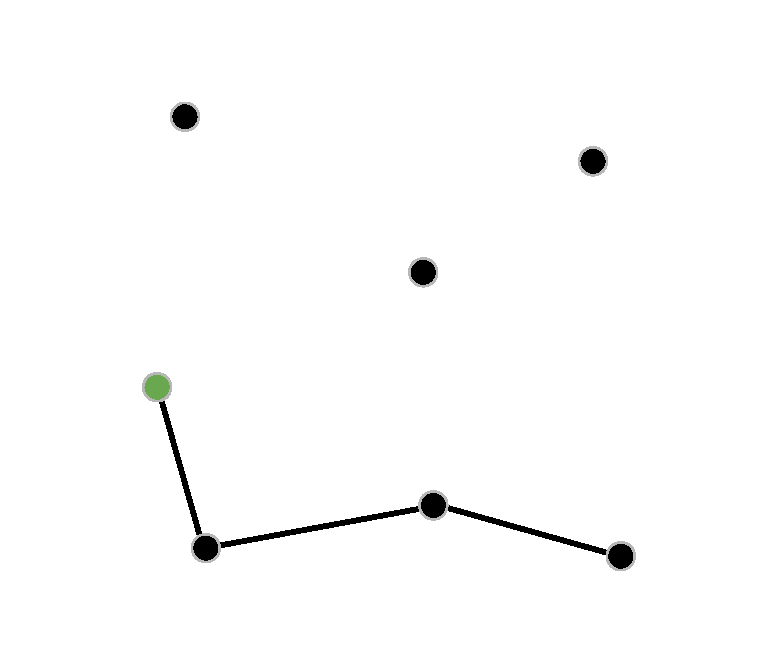
\includegraphics[width=\linewidth]{media/fase3.pdf}
    \caption{Third step}
  \end{subfigure}
  \begin{subfigure}[b]{0.49\linewidth}
    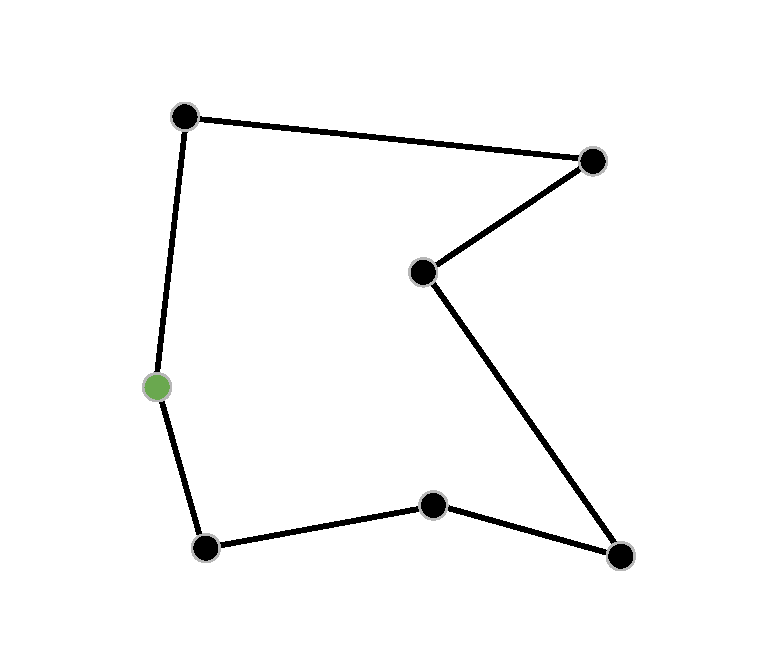
\includegraphics[width=\linewidth]{media/fase4.pdf}
    \caption{Final result}
  \end{subfigure}
  \caption{Execution of nearest neighbor algorithm}
\end{figure}

\noindent On our implementation we decided to trade space for time. Since the operation to compute the nearest point is repeated several time, we decide to store for each point the list of all others points sorted by their distances from that one. This require $O(n^2)$ additional space. Considering the time, instead, to sort the points we implemented a simple \textit{insertion sort}, that is $O(n^2)$, so in total we need an initial $O(n^3)$ (This part could be further improved with a better sort algorithm like \textit{merge sort} that is $O(n \cdot log(n))$, but since the initial time to order the nodes on our experiments was negligible, we decided to use insertion sort that was easier to implement). So, by paying this initial cost we were able to speed up each iteration of nearest neighborhood, in fact each time we needed to find the nearest point we just had to pick the first available one from the ordered list. Of course in the worst case this is $O(n)$, because it can happen that the firsts elements of the ordered list have already been visited, so I have to run across most of the list until I find an available point. However, what we saw in practice is that, except when there are left few nodes to visit, the first available element is always on the firsts position of the ordered list so the operation to find the nearest neighbor became $\Theta(1)$ in most of the cases (for example, we tried on multiple instances between 100 and 500 points and the average number of access to the ordered list to find the nearest point was between 3 and 6). \\

\noindent The major problem of this technique is that visiting always the next closest point leads to the creation of lots of intersection between edges, that of course are inefficient. A possible solution to improve this initial result will be shown on the next section dedicated to the refining algorithms. \\
Another problem is that this algorithm is deterministic, so this mean that if it is run twice starting from the same initial point, it produce the same solution. The consequence of this is that the number of different circuit that it can explore is limited to the total number of nodes.

\subsection{GRASP}
GRASP is a variation of nearest neighborhood that introduce a random component. On each iteration, rather than picking the nearest point to the last visited, select the three closest points and choose one of them at random as next visited vertex. 
(Or alternatively assign a different probability to each of the three points, for example 0.6 to the closest point and 0.3 and 0.1 respectively to the second and the third).

\begin{algorithm}
	\caption{GRASP}\label{GRASP method}
	\hspace*{\algorithmicindent} \textbf{Input:} Instance I of the TSP \\
	\hspace*{\algorithmicindent} \textbf{Output:} Admissible solution for the instance
    \begin{algorithmic}[1]
    		\State \textit{cost(bestSolution) $\leftarrow \infty$}
		\While{! termination condition}
			\State S $\leftarrow$ empty list
			\State notVisitedList $\leftarrow$ all vertices
			\State currentVertex $\leftarrow$ pick 1 random vertex from I
			\State notVisitedList $\leftarrow$ remove(currentVertex) 
			\State S $\leftarrow$ add(currentVertex)
			\For{$i = 1$, $i < N$, i++}
				\State v1, v2, v3 $\leftarrow$ pick 3 closest and not visited vertex from currentVertex
				\State nextVertex $\leftarrow$ choose at random one between v1, v2, v3
				\State notVisitedList $\leftarrow$ remove(nextVertex) 
				\State S $\leftarrow$ add(nextVertex)
				\State currentVertex $\leftarrow$ nextVertex
			\EndFor
			\If{cost(S) $<$ cost$($bestSolution$)$}
				\State bestSolution $\leftarrow$ S
			\EndIf
		\EndWhile 
		\State \textbf{return} S
    \end{algorithmic}
\end{algorithm}

\noindent Our implementation was almost the same of nearest neighborhood, with the construction for each point of the initial list of all other points sorted by their distance from that point, with the only difference that first three available points are picked from the list, rather than only one, and the next visited point is chosen at random from them. 
The introduction of the random component means that the probability to repeat the same sequence starting from the same point is very minimal, so GRASP can explore lots of different circuit resolving the problem of determinism of nearest neighborhood. 

\begin{figure}[h!]
  \centering
  \begin{subfigure}[b]{0.49\linewidth}
    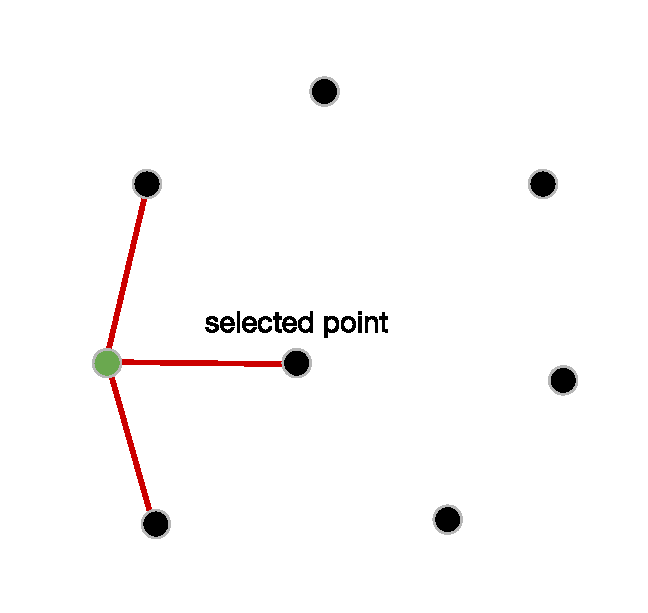
\includegraphics[width=\linewidth]{media/grasp_fase1.pdf}
     \caption{Initial step}
  \end{subfigure}
  \begin{subfigure}[b]{0.49\linewidth}
    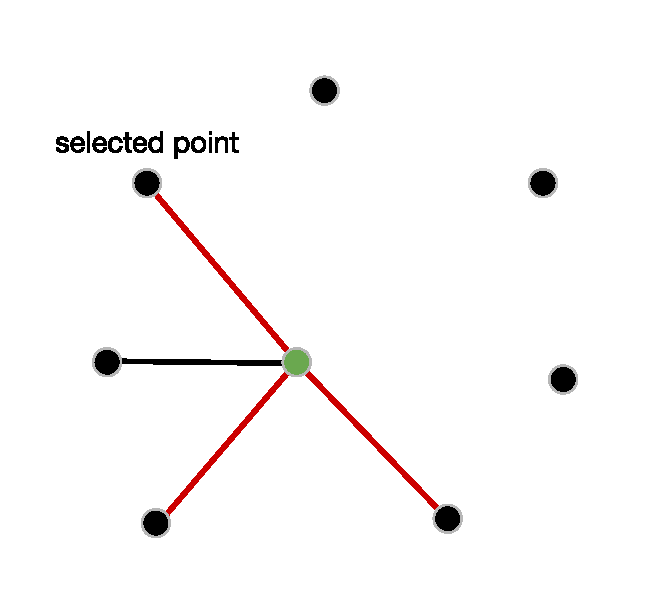
\includegraphics[width=\linewidth]{media/grasp_fase2.pdf}
    \caption{Second step}
  \end{subfigure}
  \begin{subfigure}[b]{0.49\linewidth}
    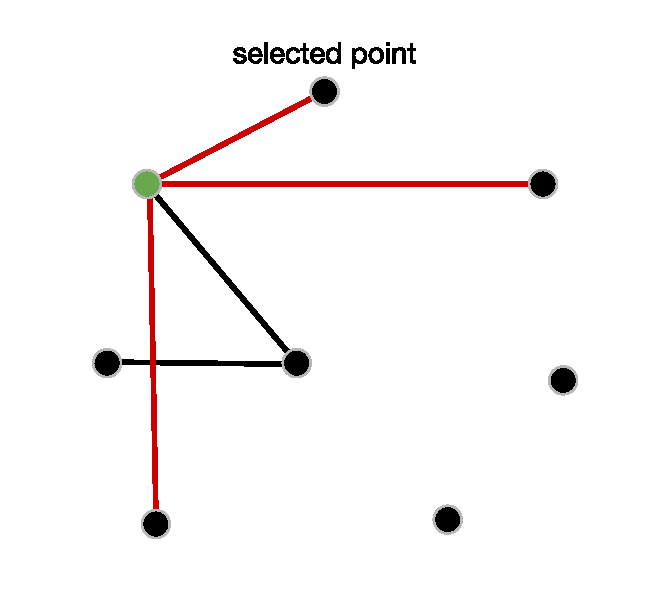
\includegraphics[width=\linewidth]{media/grasp_fase3.pdf}
    \caption{Third step}
  \end{subfigure}
  \caption{Execution of 3 steps of GRASP. Each time the 3 closest points are considered and one is picked at random.}
\end{figure}

\subsection{Insertion heuristic}
This algorithm starts from a simple circuit made with only two points. At each iteration, for each of the remaining vertices to insert, compute the minimal extra mileage. The extra mileage is the cost to insert a point on the circuit. So, for example, if we want to insert the vertex z between vertex x and vertex y, the extra mileage is: $c_{xz} + c_{zy} - c_{xy}$, where $c_{ij}$ is the cost of the edge (i, j). The fact that for each point we search the minimal extra mileage means that we are looking to the best position where insert that point. Insert vertex that has the best extra mileage into the partial circuit and repeat the procedure until all the points are inserted (Figure \ref{fig:insertion}). The algorithm than can be executed several time to explore new solutions, starting every time from different initial points and updating the incumbent if necessary. \\
The cost to compute the best extra mileage is $O(n^2)$, so this mean that the entire algorithm is $O(n^3)$.\\
It is also possible to add the GRASP rule, so rather then selecting the point with the best extra mileage, find the three smallest extra mileages and choose at random between them, in this way the algorithm doesn't converge to the same solution starting from the same initial circuit. \\

\begin{algorithm}
	\caption{Insertion heuristic}\label{Insertion method}
	\hspace*{\algorithmicindent} \textbf{Input:} Instance I of the TSP \\
	\hspace*{\algorithmicindent} \textbf{Output:} Admissible solution for the instance
    \begin{algorithmic}[1]
    		\State \textit{cost(bestSolution) $\leftarrow \infty$}
		\While{! termination condition}
			\State S $\leftarrow$ empty list
			\State S $\leftarrow$ add 2 initial vertices
			\While{! all point are inserted}
				\State bestExtraMileage $\leftarrow \infty$
				\For{\textbf{each} point p to insert}
					\State minExtraMileage $\leftarrow \infty$
					\For{\textbf{each} edge e $\in$ S}
						\State extraMileage $\leftarrow$ computeExtraMileage(p, e)
						\If{extraMileage $<$ minExtraMileage}
							\State minExtraMileage $\leftarrow$ extraMileage
						\EndIf
					\EndFor
					\If{minExtraMileage $<$ bestExtraMileage}
						\State bestExtraMileage $\leftarrow$ minExtraMileage
					\EndIf
				\EndFor
				\State S $\leftarrow$ insert point with bestExtraMileage in the best poisiton
			\EndWhile
			\If{cost(S) $<$ cost(bestSolution)}
				\State bestSolution $\leftarrow$ S
			\EndIf
		\EndWhile 
		\State \textbf{return} bestSolution
    \end{algorithmic}
\end{algorithm}

\begin{figure}[h!]
  \centering
  \begin{subfigure}[b]{0.49\linewidth}
    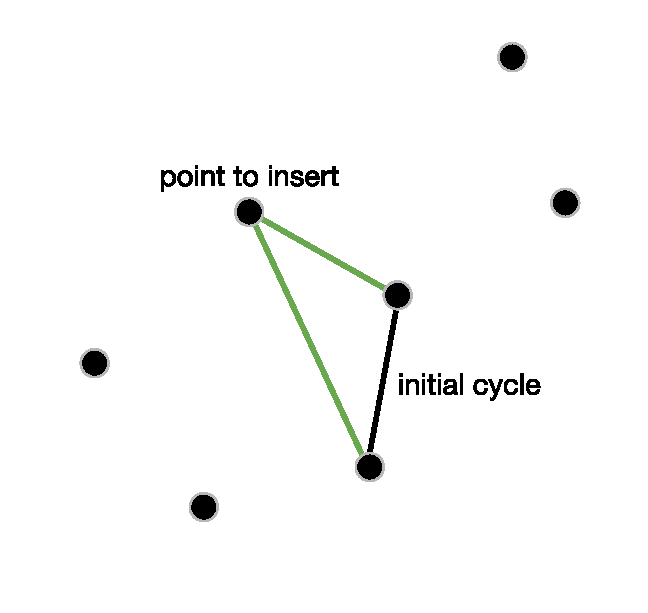
\includegraphics[width=\linewidth]{media/insertion1.pdf}
     \caption{Initial step}
  \end{subfigure}
  \begin{subfigure}[b]{0.49\linewidth}
    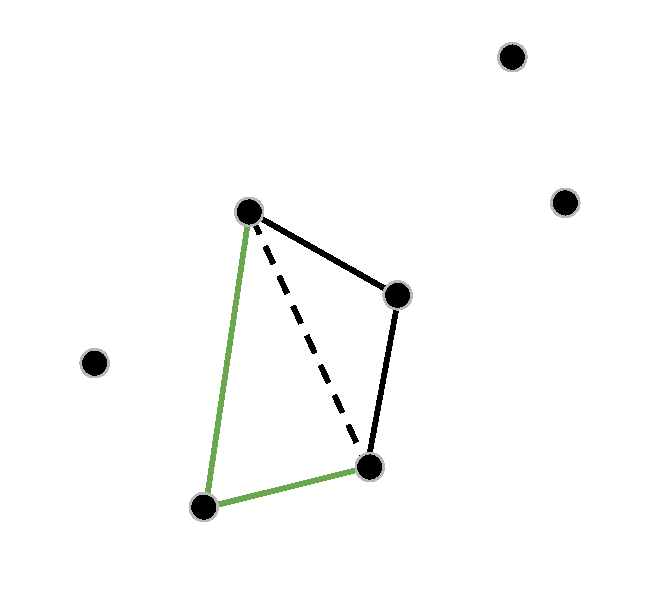
\includegraphics[width=\linewidth]{media/insertion2.pdf}
    \caption{Second step}
  \end{subfigure}
  \begin{subfigure}[b]{0.49\linewidth}
    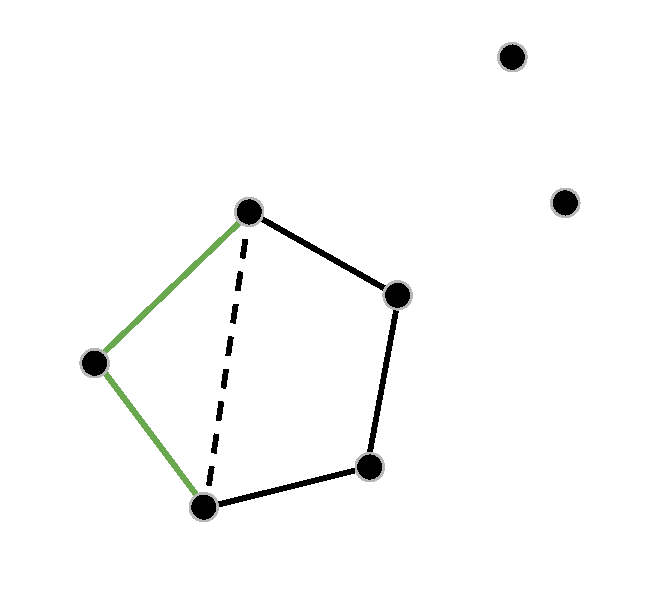
\includegraphics[width=\linewidth]{media/insertion3.pdf}
    \caption{Third step}
  \end{subfigure}
  \begin{subfigure}[b]{0.49\linewidth}
    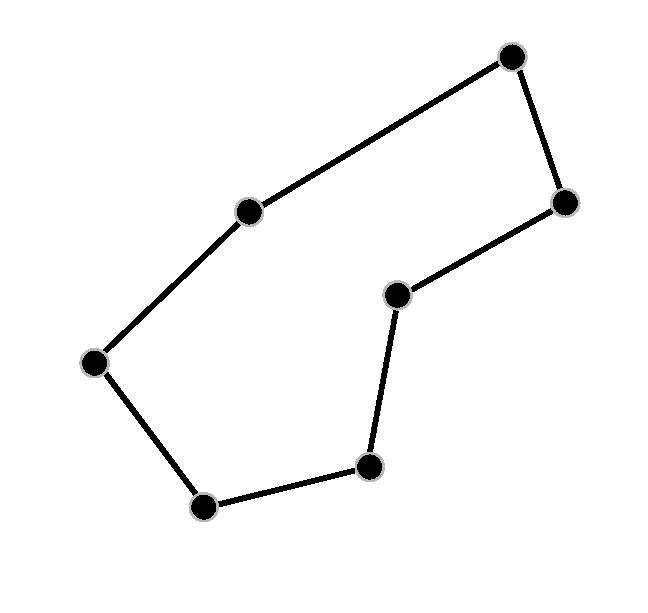
\includegraphics[width=\linewidth]{media/insertion4.pdf}
    \caption{Final result}
  \end{subfigure}
  \caption{Execution of insertion heuristic algorithm}
  \label{fig:insertion}
\end{figure}

\noindent On our implementation to select the initial circuit we decided to pick at random one point and then to select the furthest point from that one. (Of course this is not the only solution: other possibility are, for example, to pick a vertex and its closest one, or to choose two points completely at random.) I addition, at the beginning of the algorithm, we built a matrix where the element i j contains the distance between vertices i and j (So in total we payed an additional $O(n^2)$ in space). We made this choice because on this algorithm distances between points are computed several times and in addition the same distance can be calculated more than once.\\


\subsection{Insertion with convex hull}
This is a variation of the insertion algorithm. It works in the same way but the initialization is different: rather than starting from an initial cycle made of two random points, compute the convex hull \footnote{In geometry, the convex hull or convex envelope or convex closure of a shape is the smallest convex set that contains it, \url{https://en.wikipedia.org/wiki/Convex_hull}.
} of the instance. Then iterate and insert all the remaining points, that are all inside the convex hull, in the same way of Insertion heuristic (Figure \ref{fig:insertionHull}).\\
On our implementation, to find the initial convex hull, we used the Graham Scan algorithm, freely provided by the website www.geeksforgeeks.org. This algorithm is $O(n \cdot log(n))$ and it is performed only once at the beginning so it doesn't impact the overall execution time for the insertion that is $O(n^3)$ as explained on the previous subsection. For more information about the Graham Scan consult \url{https://www.geeksforgeeks.org/convex-hull-set-2-graham-scan/}.

\begin{figure}[h!]
  \centering
  \begin{subfigure}[b]{0.8\linewidth}
    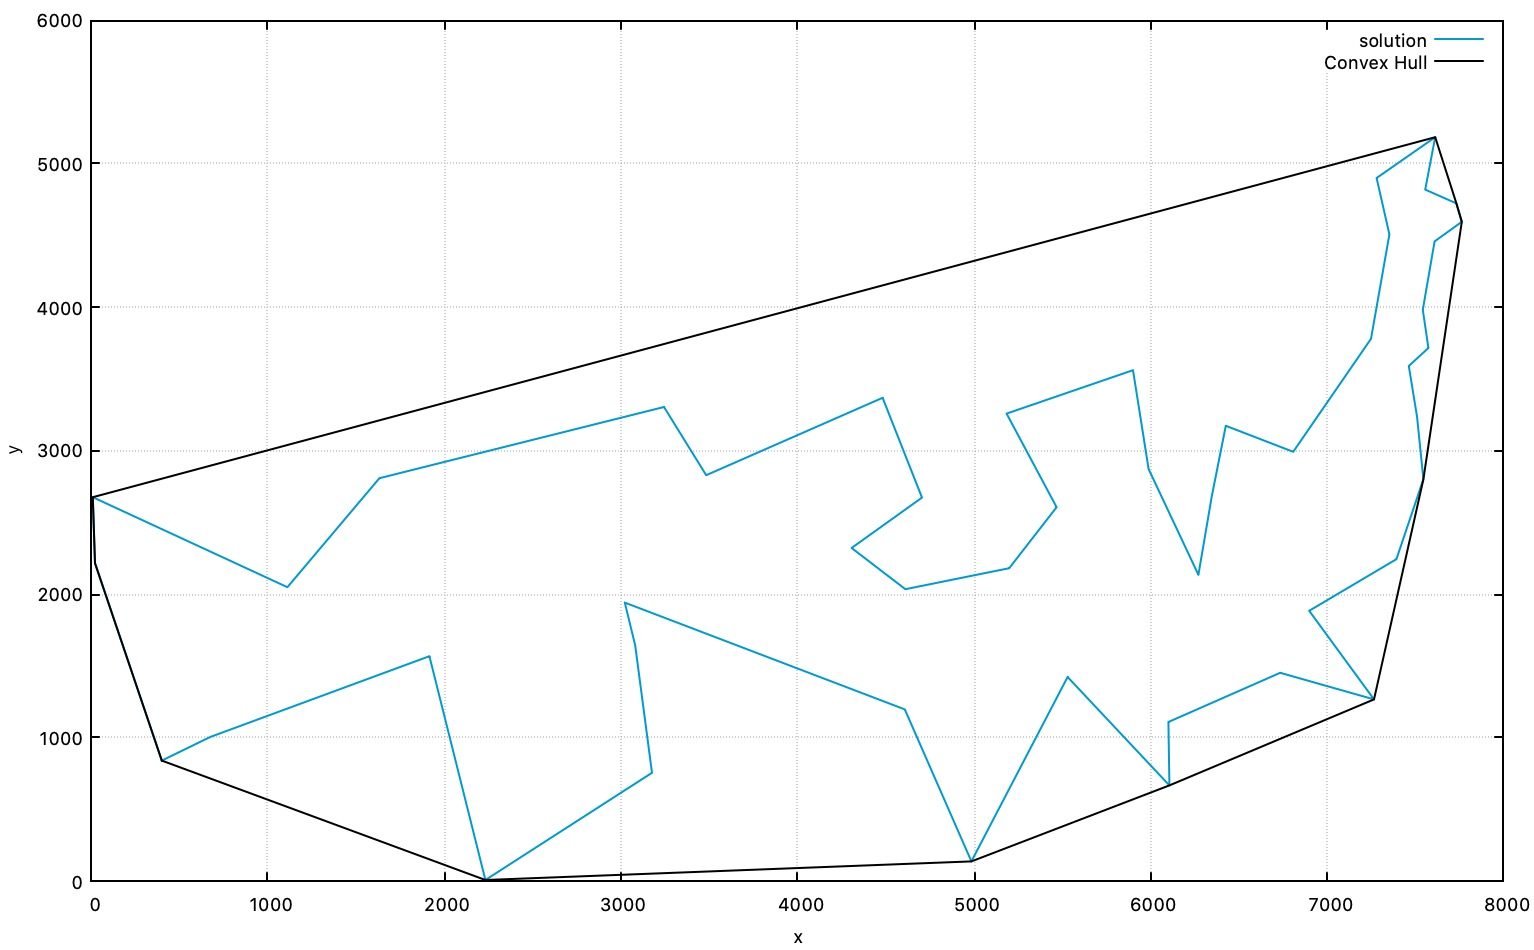
\includegraphics[width=\linewidth]{media/convex1.jpg}
     \caption{problem att48}
  \end{subfigure}
  \begin{subfigure}[b]{0.8\linewidth}
    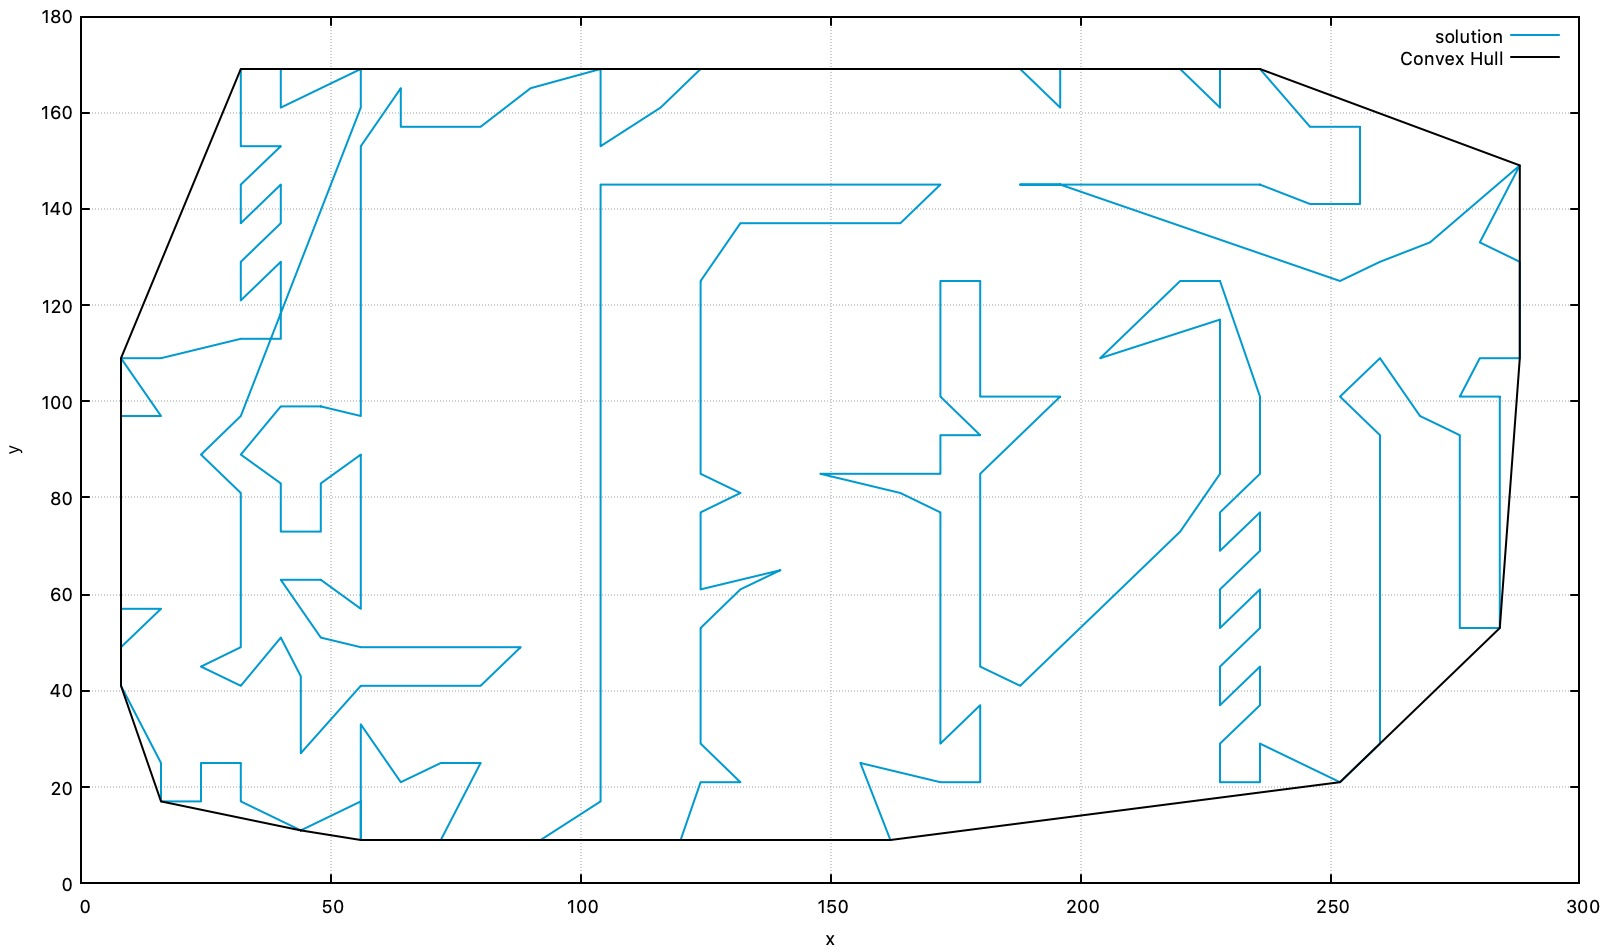
\includegraphics[width=\linewidth]{media/convex2.jpg}
    \caption{problem a280}
  \end{subfigure}
  \caption{Execution of the insertion with convex hull on 2 different problems. It is possible to see the initial convex hull and the final result when all the points inside it are inserted}
  \label{fig:insertionHull}
\end{figure}

\subsection{Final comparison between solution builder}

\begin{figure}[h!]
	\centering
	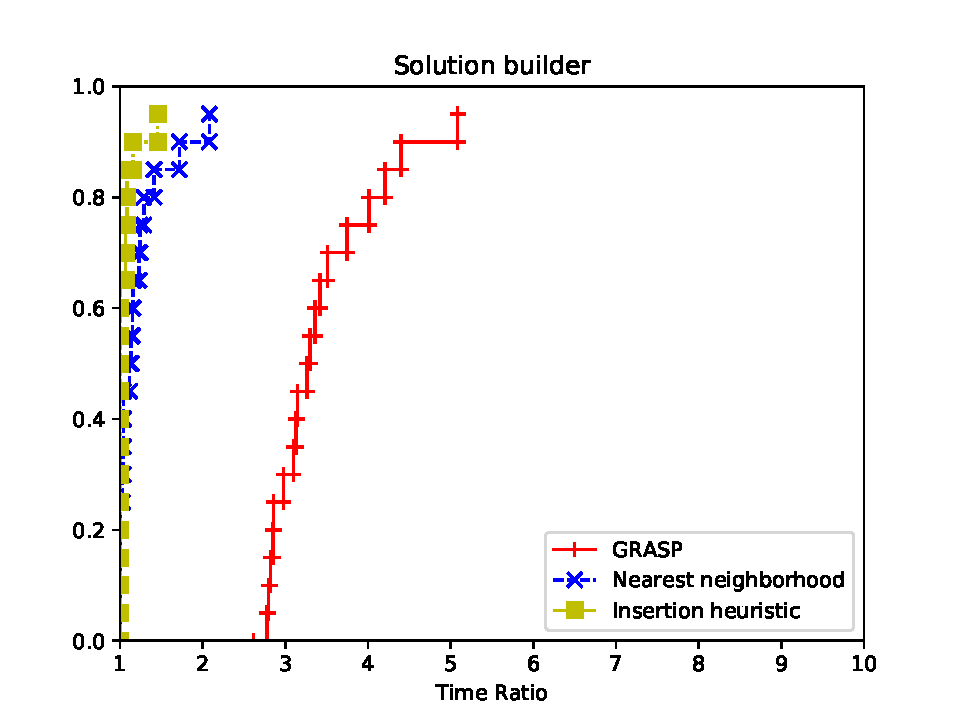
\includegraphics[scale=0.8]{media/builder.pdf}
	\caption{Performance profile of the solution builders}
	\label{fig:solbuilder}
\end{figure}
\noindent
On Figure \ref{fig:solbuilder} the final confrontation between the heuristic solution builders. To obtain these result we test the algorithms on the dataset of 20 instances with a time limit of 5 minutes. 

\clearpage
%\newpage

\section{Refining algorithms}
Refining algorithm are so called because they start from an admissible solution that could by provided by any other algorithm and they try to improve it with a series of iteration.

\subsection{TWO-OPT}
The first algorithm we present is TWO-OPT (or 2-OPT). To explain this technique, let's consider two edges, the first delimited by vertices a and b and with cost $c_{ab}$, the second delimited by c and d and with cost $c_{cd}$ (Both edges belong to an admissible solution provided by any algorithm). Now let's remove these edges and reconnect the vertices in a different way: as result we obtain the edges a, c and b, d with cost respectively $c_{ac}$ and $c_{bd}$. Now lets compute: 
\begin{equation*}
\Delta = c_{ab} + c_{cd} - (c_{ac} + c_{bd})
\end{equation*}
that is the cost of the initial removed edges minus the cost of the new edges. If $\Delta > 0$, it means that the new edges are better than the older and the swap is worth because it reduce (improve) the objective function. Of course the new solution produced is still admissible (Figure \ref{fig:twoopt}).\\

\begin{figure}[h!]
\centering
	\begin{tabular}{@{}cccc@{}}
		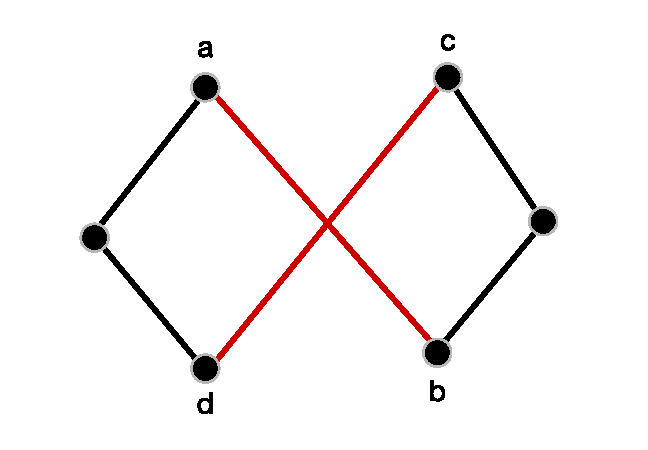
\includegraphics[scale=0.6]{media/twopt1.pdf} &
		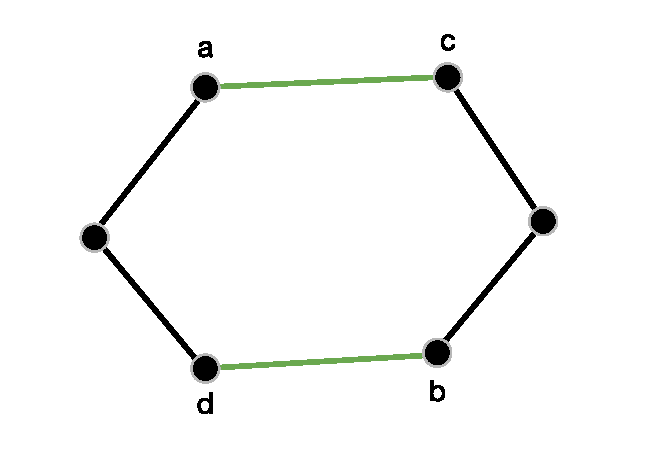
\includegraphics[scale=0.6]{media/twopt2.pdf} \\
	\end{tabular}
	\caption{The 2-OPT move, edges in red are removed and replaced by green edges.}
	\label{fig:twoopt}
\end{figure}

\noindent 2-OPT works in this way: start from an admissible solution, consider all the possible couple of edges (that are in total $O(n^2)$) and for each of them compute the $\Delta$ (That can be calculated in $\Theta(1)$). Then pick the largest $\Delta$, remove the relative edges and reconnect the vertices as previously explained. After this operation, one of the two parts of the cycle that has been divided by the swap, need to be retraced in order to invert the visit sequence of the vertices and reconnect it to the new edge (This is $O(n)$, but since it is done after a $O(n^2)$ doesn't change the overall cost of the swap). Repeat the procedure until all the $\Delta$ are negative, or a fixed time limit is reached.\\

\begin{algorithm}
	\caption{2-OPT}\label{2-OPT method}
	\hspace*{\algorithmicindent} \textbf{Input:} Admissible solution S \\
	\hspace*{\algorithmicindent} \textbf{Output:} Best solution found
    \begin{algorithmic}[1]
		\While{! termination condition}
			\State best$\Delta \leftarrow \infty$
			\For {\textbf{each} couples of edge $v_{ab}$, $v_{cd} \in S$}
				\State $\Delta \leftarrow c_{ab} + c_{cd} - (c_{ac} + c_{bd})$ 
				\If{$\Delta < Best\Delta$}
					\State best$\Delta \leftarrow \Delta$
				\EndIf
			\EndFor
			\If{best$\Delta > 0$}
				\State $S \leftarrow$ perform move with best$\Delta$
			\Else
				\State \textbf{return} S
			\EndIf
		\EndWhile
		\State \textbf{return} S
    \end{algorithmic}
\end{algorithm}

\noindent On our implementation we followed the procedure described above, with the addition of a matrix to store all the distances between points, to avoid to recompute them more than once.\\
This algorithm is very good to remove edge intersections, like the ones produced  by nearest neighborhood (or GRASP). Here in Table \ref{tab:twoopt} some examples.\\ 

\begin{table}[h!]
	\begin{center}
		\begin{tabular}{l|c|c|c}
			\textbf{Instance} & \textbf{GRASP} & \textbf{2-OPT} & \textbf{Improve}	\\
			& (5 sec) & (5 sec) & \\
			\hline
			att48 & 41806 & 35522 & 15\% \\
			eil101 & 879 & 691 & 21\% \\
			ch130 & 9801 & 6347 & 35\% \\
			ch150 & 10477 & 7278 & 30\% \\
			a280 & 4546 & 2886 & 36\% \\
			lin318 & 76940 & 46235 & 39\% \\ 
			att532 & 155010 & 97487 & 37\% \\	
			pr1002 & 492311 & 285078 & 42\% \\
		\end{tabular}
		\caption{Values of the objective functions after running on each instance GRASP algorithm for 5 seconds and then 2-OPT for other 5 seconds.}
		\label{tab:twoopt}
	\end{center}
\end{table}

\noindent These results were obtained after running GRASP for five seconds and then refining the solution with 2-OPT for other five seconds. Of course this dataset is very small but it gives the idea of the power of this technique, we have, in fact, a significant improve of the objective function in all the cases. To notice that the improve increase with large problem. \\
It is possible to visualize the action of 2-OPT by plotting the solution before and after the refining like in Figure \ref{fig:grasp}.

\begin{figure}[h!]
\centering
	\begin{tabular}{@{}cccc@{}}
		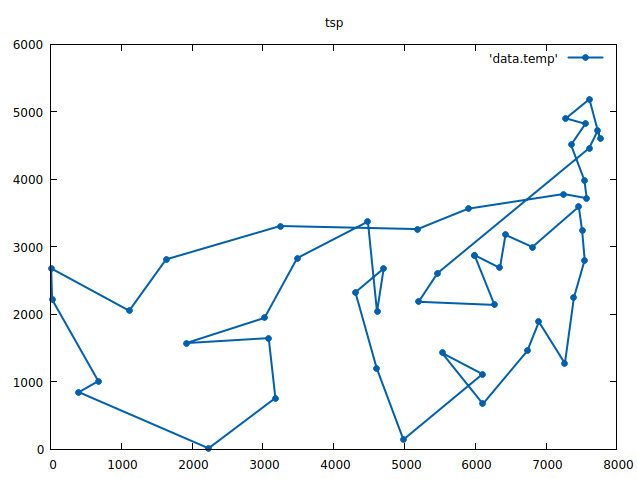
\includegraphics[scale=0.5]{media/before2opt.png} \\
		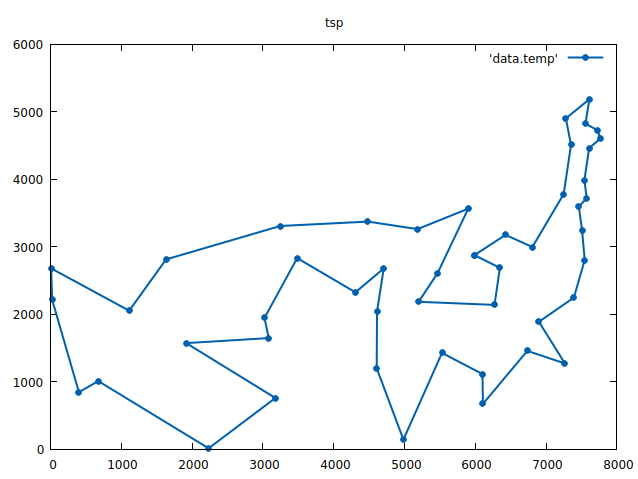
\includegraphics[scale=0.5]{media/after2opt.png} \\
	\end{tabular}
	\caption{Solution of 5 sec of GRASP before (top image) and after (bottom image) a refining of 5 sec}
	\label{fig:grasp}
\end{figure}


\subsection{THREE-OPT}
3-OPT is a variation of 2-OPT that consider 3 edges for the swap rather than only two. This time there are multiple way to reconnect the vertices of the 3 removed edges, in particular for a triad there are 7 possible moves (Figure  \ref{fig:threeopt}). Moreover, we have to consider all the possible triad to find the best one and this is $O(n^3)$. So in general 3-OPT is more complicated to implement and due to the fact that is cubic doesn't work well with big problems, for example with instances with more than 10000 points.

\begin{figure}[h!]
  \centering
  \begin{subfigure}[b]{0.24\linewidth}
    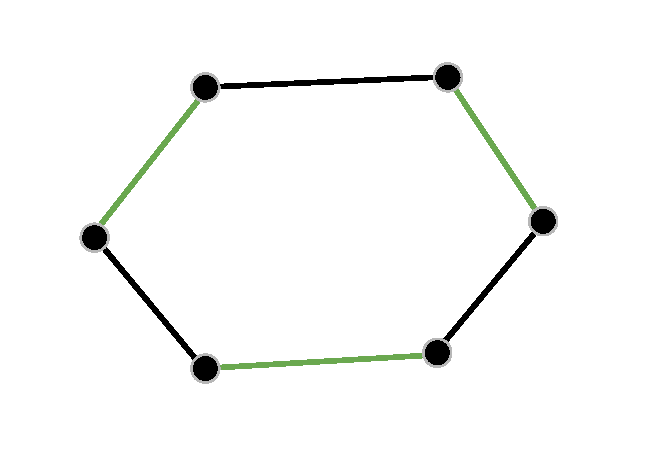
\includegraphics[width=\linewidth]{media/threeopt1.pdf}
     \caption{}
  \end{subfigure}
  \begin{subfigure}[b]{0.24\linewidth}
    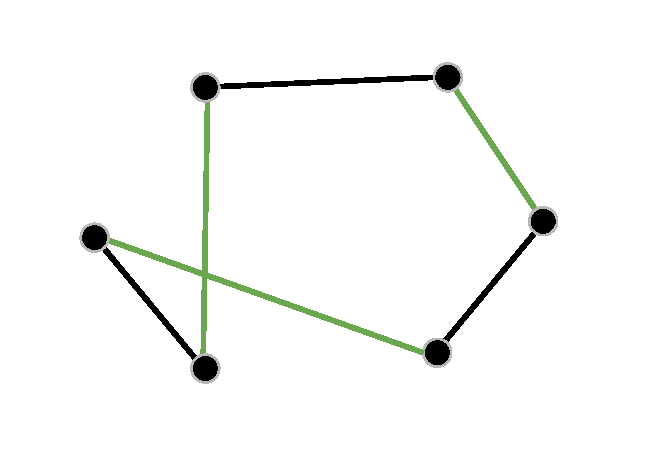
\includegraphics[width=\linewidth]{media/threeopt2.pdf}
    \caption{}
  \end{subfigure}
  \begin{subfigure}[b]{0.24\linewidth}
    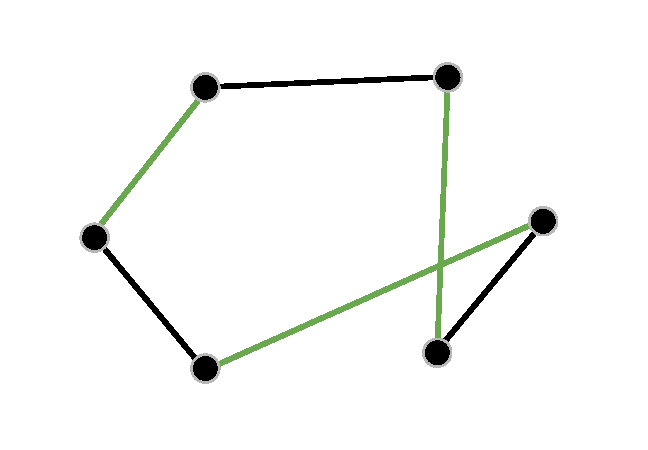
\includegraphics[width=\linewidth]{media/threeopt3.pdf}
    \caption{}
  \end{subfigure}
  \begin{subfigure}[b]{0.24\linewidth}
    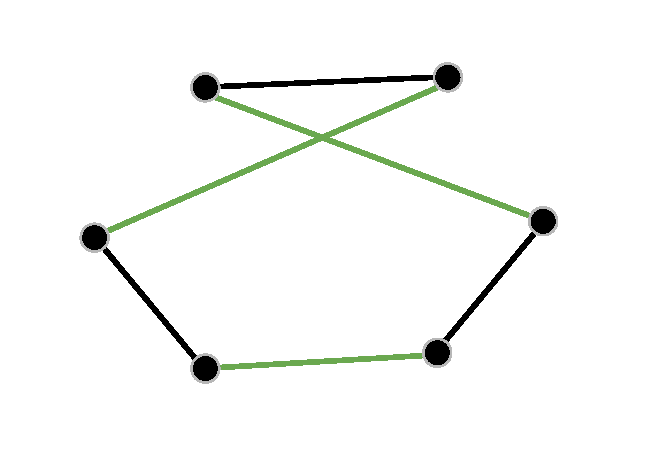
\includegraphics[width=\linewidth]{media/threeopt4.pdf}
    \caption{}
  \end{subfigure}
  \begin{subfigure}[b]{0.24\linewidth}
    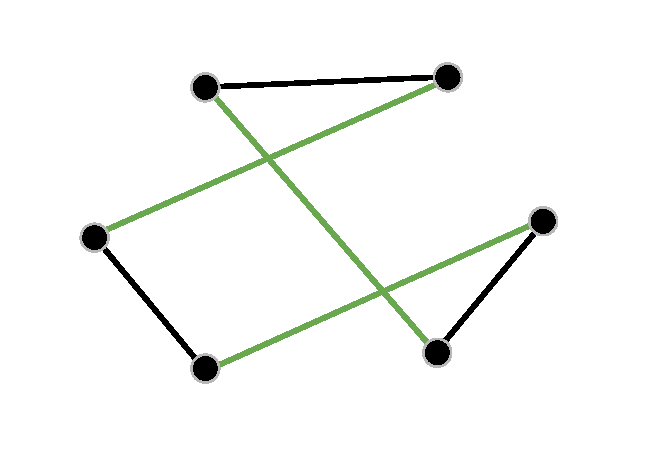
\includegraphics[width=\linewidth]{media/threeopt5.pdf}
     \caption{}
  \end{subfigure}
  \begin{subfigure}[b]{0.24\linewidth}
    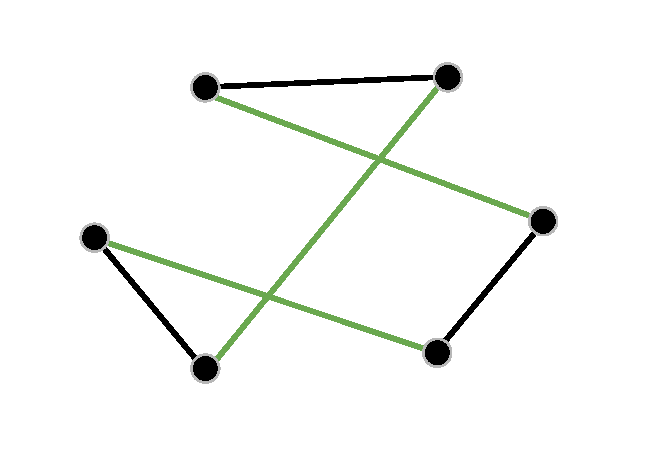
\includegraphics[width=\linewidth]{media/threeopt6.pdf}
    \caption{}
  \end{subfigure}
  \begin{subfigure}[b]{0.24\linewidth}
    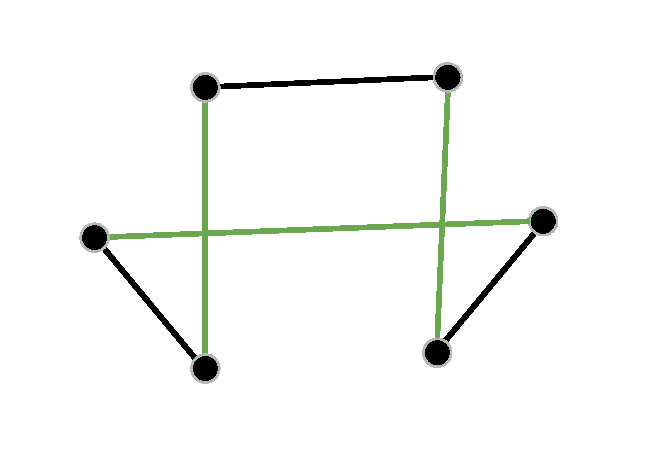
\includegraphics[width=\linewidth]{media/threeopt7.pdf}
    \caption{}
  \end{subfigure}
  \begin{subfigure}[b]{0.24\linewidth}
    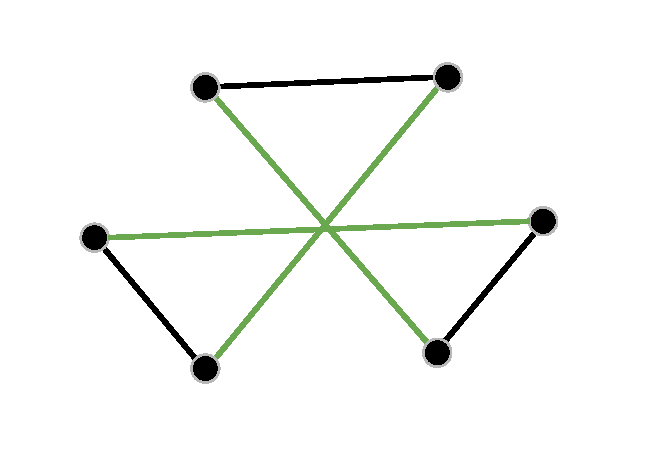
\includegraphics[width=\linewidth]{media/threeopt8.pdf}
    \caption{}
  \end{subfigure}
  \caption{All the possible 3-OPT moves given a triad of edges.}
  \label{fig:threeopt}
\end{figure}
 
\noindent We also repeated the same experiment we did for the 2-OPT, so we run on different problems GRASP for 5 seconds and then 3-OPT on the result for other 5 second. The results are shown on Table \ref{tab:threeopt}. Again the dataset is small because the only goal was to show the power of this refinement algorithm and not to compare it with other techniques. Observing the table we can notice that the improve for the smaller problems is almost the same, or sometimes better than the one with 2-OPT, but more importantly we can notice that the algorithm scales bad with big problems due to the fact that it's cubic. In fact 5 seconds is a relatively small amount of time and in this short period the number of 3-OPT moves that the algorithm is able to perform is small so the improve is poor.

\begin{table}[h!]
	\begin{center}
		\begin{tabular}{l|c|c|c}
			\textbf{Instance} & \textbf{GRASP} & \textbf{3-OPT} & \textbf{Improve}	\\
			& (5 sec) & (5 sec) & \\
			\hline
			att48 & 42086 & 33588 & 20\% \\
			eil101 & 875 & 665 & 25\% \\
			ch130 & 9894 & 6373 & 35\% \\
			ch150 & 10503 & 6828 & 35\% \\
			a280 & 4588 & 3247 & 29\% \\
			lin318 & 75526 & 56496 & 25\% \\ 
			att532 & 153954 & 144295 & 6\% \\	
			pr1002 & 487157 & 481381 & 1\% \\
		\end{tabular}
		\caption{Values of the objective functions after running on each instance GRASP algorithm for 5 seconds and then 3-OPT for other 5 seconds.}
		\label{tab:threeopt}
	\end{center}
\end{table}

\newpage

\section{Metaheuristics}
A metaheuristic is a higher-level procedure or heuristic designed to find, generate, or select a heuristic (partial search algorithm) that may provide a sufficiently good solution to an optimization problem, especially with incomplete or imperfect information or limited computation capacity \cite{meta}.

\subsection{Multi-start}
After performing a refinement technique, like 2-OPT, if the time limit is not reached, the algorithm stop on a local minima of the objective function. Of course at this point we want to escape from this local minima and search for a better one that hopefully is also the optimum. A possible solution is the multi-start approach, so each time we restart from the beginning, providing another initial solution and refining it. On each iteration, if the algorithm that provide the initial solution is well randomized (like GRASP) we will stop on a different local minima. So we can keep track of the best one and return it when the time limit for this procedure is reached.
The main problem of this technique is that is not very efficient because each time I restart all the information we obtained on the previous local minima is unused.
More powerful technique will be shown on the following subsections.

\subsection{Variable neighborhood search}
Variable neighborhood search (VNS) provide a simple yet powerful way to escape the local minima. Let's assume that we have completed the refinement using 2-OPT. At this point we can perform a random move with a bigger research radius, like a 3-OPT or a 5-OPT for example. Since this move is completely random, it will make the solution worse but it will also provide the ``kick" that we need to escape the local minima. Now we can restart with 2-OPT until a new minima is found (that could also be the optimum).\\
In synthesis, VNS, works with two phases that alternate continuously: an intensification  phase (2-OPT) where the algorithm move toward a minima and a diversification phase where VNS perform a k-OPT random move to exit from the minima.

\begin{algorithm}
	\caption{VNS}\label{VNS method}
	\hspace*{\algorithmicindent} \textbf{Input:} Admissible solution S \\
	\hspace*{\algorithmicindent} \textbf{Output:} Best solution found
    \begin{algorithmic}[1]
    		\State \textit{bestSolution $\leftarrow$ S}
		\While{! termination condition}
			\State bestMove $\leftarrow$ find best 2-OPT move of S
			\If{$\Delta($bestMove$) > 0$}
				\State S $\leftarrow$ perform bestMove
			\Else
				\State S $\leftarrow$ perform random k-OPT move
			\EndIf
			\If{cost$($S$)$ $<$ cost$($bestSolution$)$}
				\State bestSolution $\leftarrow S$
			\EndIf
		\EndWhile
		\State \textbf{return} bestSolution
    \end{algorithmic}
\end{algorithm}

\begin{figure}[h!]
\centering
	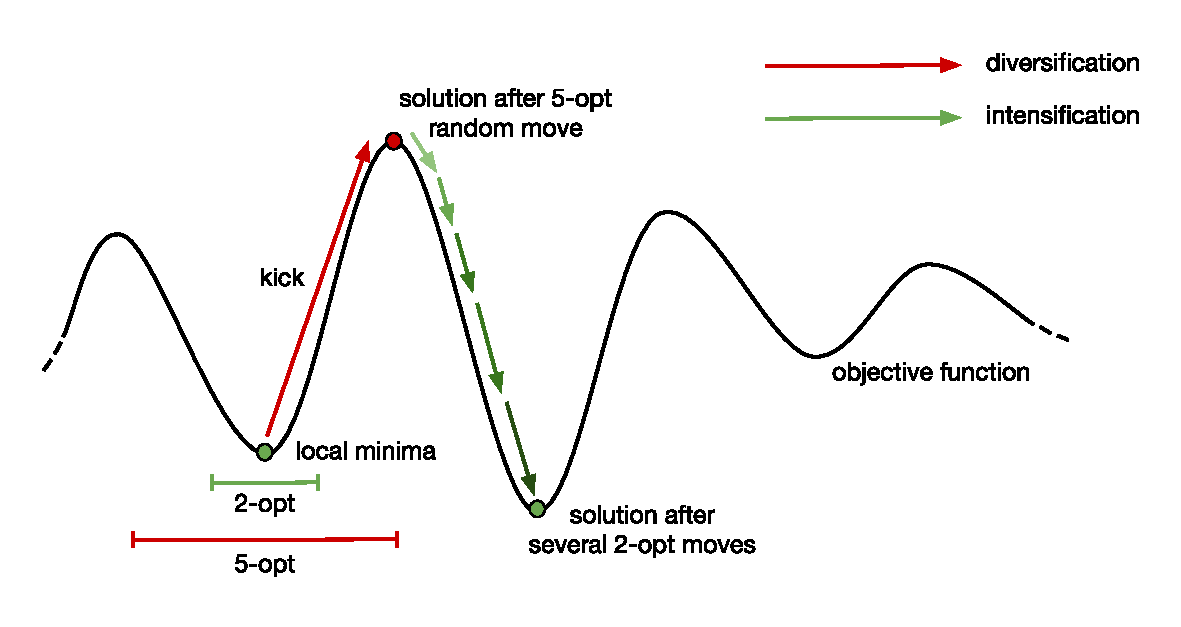
\includegraphics[scale=0.77]{media/vns_graph.pdf} \\
	\caption{Representation of an objective function during VNS and the ``kick" of a 5-OPT random move}
\end{figure}

\noindent On our implementation we use the technique showed in Figure \ref{fig:vns}. We select the edges to remove (that in our example are three) and then we reconnect the vertices in a specific way, so that the reversal of some edges to reconstruct the cycle (the one described in 5.2.1) is never required. In particular, because we can assign to the cycle a direction of travel, for each edge that we want to remove we can distinguish an initial vertex (the ones in red) and a final vertex (the ones in green). The idea is to always reconnect an initial vertex to a final vertex so the direction of travel is preserved. So for example we can start from the initial vertex of the first edge to remove and connect it to the final vertex of the second edge to remove. Then we pick the initial vertex of the second edge and we connect it to the final vertex of the third and so on, until the cycle is reconstructed. Of course this is valid for k edges, so on our implementation we can perform a k-opt random move, where k is establish at the beginning of the execution.

\begin{figure}[h!]
  \centering
  \begin{subfigure}[b]{0.49\linewidth}
    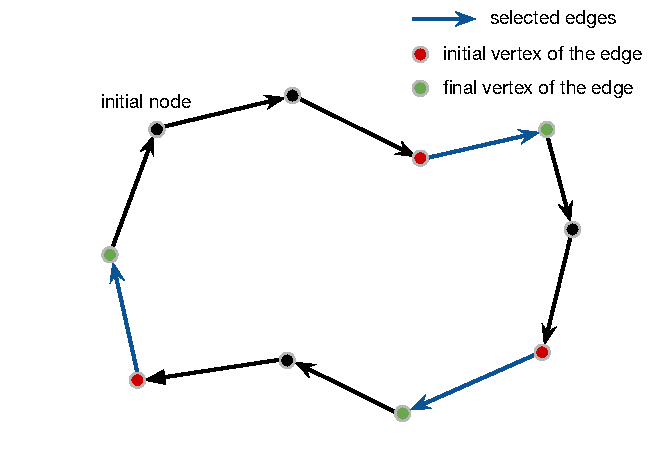
\includegraphics[width=\linewidth]{media/vnss12.pdf}
     \caption{}
  \end{subfigure}
  \begin{subfigure}[b]{0.49\linewidth}
    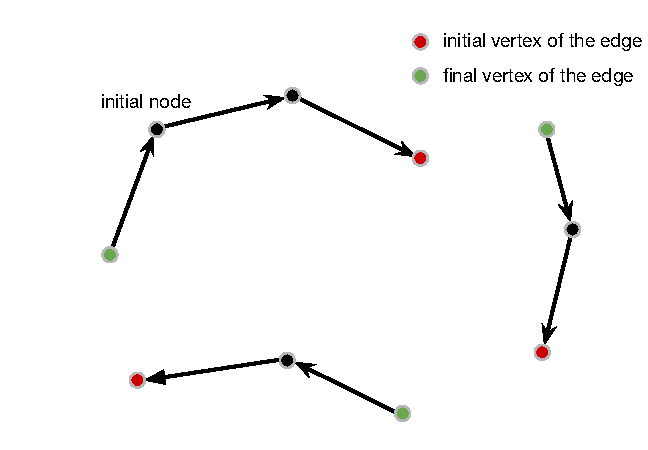
\includegraphics[width=\linewidth]{media/vnss22.pdf}
    \caption{}
  \end{subfigure}
  \begin{subfigure}[b]{0.49\linewidth}
    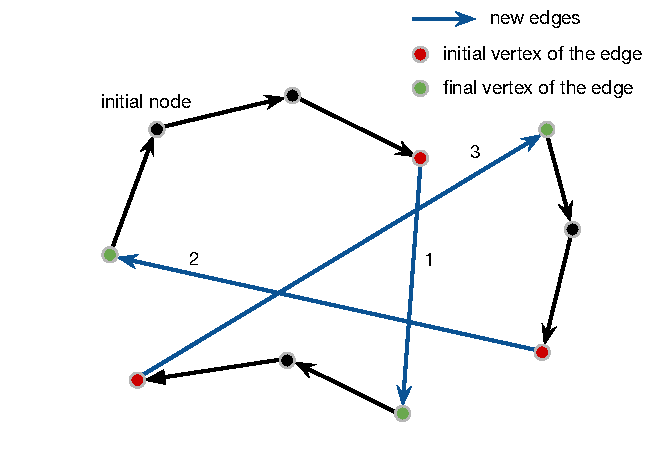
\includegraphics[width=\linewidth]{media/vnss32.pdf}
    \caption{}
  \end{subfigure}
  \caption{Passages for a k-OPT random move (In this case a 3-OPT move).}
  \label{fig:vns}
\end{figure}


\subsection{Tabu search}
Created by Fred W. Glover during the 80s, Tabu search provide an alternative procedure to VNS to escape from local minima. Let's assume that we have performed a refinement and we have reached a local minima, let's call this solution $x_k$. At this point, every 2-OPT move will make the objective function worse. So we choose and perform the least pejorative move, obtaining the solution $x_{k+1}$. Now, if we make another move following the 2-OPT rule, the algorithm will return to the solution $x_{k}$ by simply swapping again the edges used on the last step, cause this is the only move that improve the objective function. To avoid this, the idea is to insert these edges on a tabu list that is a list of edges that cannot be used for a 2-OPT move. This means that the move from $x_{k}$ to $x_{k+1}$ became forbidden. So we repeat this last step, performing the least pejorative move and each time inserting the edges used in the tabu list, until we reach a point where the objective function will return to improve. Of course we don't insert edges into the tabu list if the move is not pejorative. \\
To describe the algorithm we asserted that the tabu list is made of couples of edges, but this was only for a description purpose. In fact the general idea for this algorithm is that the tabu list can be made of any element that prevent to return back after a pejorative move. So for the TSP problem we can use, for example, couples of edges, a single edge or a single point. \\

\begin{algorithm}
	\caption{Tabu search}\label{TabuSearch method}
	\hspace*{\algorithmicindent} \textbf{Input:} Admissible solution S \\
	\hspace*{\algorithmicindent} \textbf{Output:} Best solution found
    \begin{algorithmic}[1]
    		\State \textit{bestSolution $\leftarrow$ S}
		\While{! termination condition}
			\If{tabuList is full}
				\State tabuList $\leftarrow$ empty list
			\EndIf
			\State bestMove $\leftarrow$ find best and not forbidden 2-OPT move of S
			\If{$\Delta($bestMove$) >$ 0}
				\State S $\leftarrow$ perform bestMove
			\Else
				\State S $\leftarrow$ perform bestMove
				\State tabuList $\leftarrow$ add(bestMove)
			\EndIf
			\If{cost$($S$)$ $<$ cost$($bestSolution$)$}
				\State bestSolution $\leftarrow S$
			\EndIf
		\EndWhile
		\State \textbf{return} bestSolution
    \end{algorithmic}
\end{algorithm}

\noindent The handle of the tabu list is very important and different strategies can have a big impact on the algorithm. Of course if we continue inserting element we will reach a point where there aren't possible moves. So we limit the size of the tabu list. The size is called tenure. When the list is full, the older element are removed.
The tenure is another parameter to set. A possible way to do this is to set a minimal and a maximal value and let the tenure oscillate among them during the algorithm. So we will have diversification phases when the tenure is big and there are lot of forbidden move and intensification phases when the tenure is small and the algorithm has lot of freedom. This is called reactive tabu search.
Another shrewdness is that if we encounter a move that is forbidden but that improves the incumbent, we will not perform that move but we will update the value of the incumbent in any case (Aspiration criterion).\\

\begin{figure}[h!]
\centering
	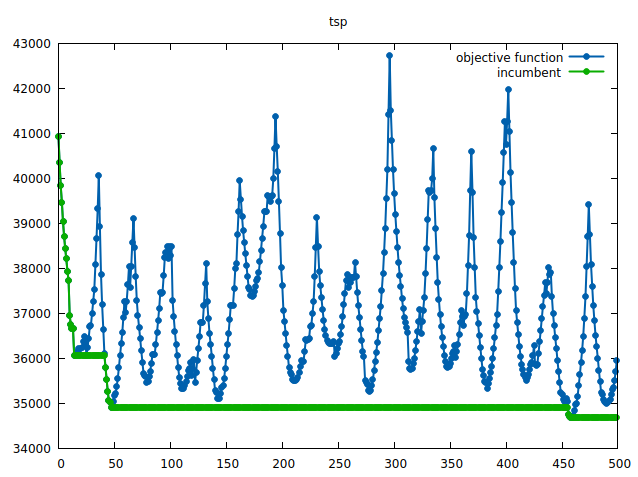
\includegraphics[scale=0.6]{media/tabuSearch1.png} \\
	\caption{Objective function and incumbent during the execution of tabu search}
\end{figure}

\noindent On our implementation we use a fixed-size tabu list, with the tenure that is a parameter decided by the user. The list records only one vertex involved in the move: so for example if we perform a pejorative move and we substitute the edges $v_{ab}$ and $v_{cd}$ with $v_{ac}$ and $v_{bd}$, only the vertex a is stored in the tabù list. When we find a good move, we check that all the 4 vertices involved are not in the tabu list, so even if we record only one point per move, this is sufficient to avoid to return back after a pejorative move. 
The check if a move is forbidden require a $O(k)$, where k is the tenure. So we perform this control only to moves that are better than the best move found until that moment (It's useless to check pejorative moves or moves that are not candidate to be selected as best move). \\
Finally we also implemented the aspiration criterion, so if a forbidden move leads to an improve of the incumbent, we keep that solution and we update the incumbent too.


\subsection{Simulated Annealing}
This metaheuristic algorithm take inspiration from the annealing technique in metallurgy that consist on heating the material and then cooling it in a controlled way. When the temperature of the materials is high, the atoms inside it it vibrates and move in a chaotic way. As the temperature decreases, the atoms reduce their state of agitation until a stable point is reached. \\
The simulated annealing works in a similar way. Let's establish a parameter, the temperature T, that initially has an high value that gradually reduce during the iterations of the algorithm. The algorithm starts from an already provided solution. On each iteration we perform a random 2-OPT (or 3-OPT) move that of course can be also pejorative. The fundamental idea is that the probability to accept the move is related to the temperature: when T is high, the system is chaotic and we accept with high probability all the random move. As the system get cooler we increase the probability to reject a bad move (so we increase the probability to perform a good move). When the temperature is close to 0, we only make meliorative moves until we reach a minima.\\
Considering the objective function, we have that, when T is high, the algorithm is randomly exploring solutions. Only when T became low the algorithm moves toward a minima that hopefully is the optimum.

\begin{figure}[h!]
\centering
	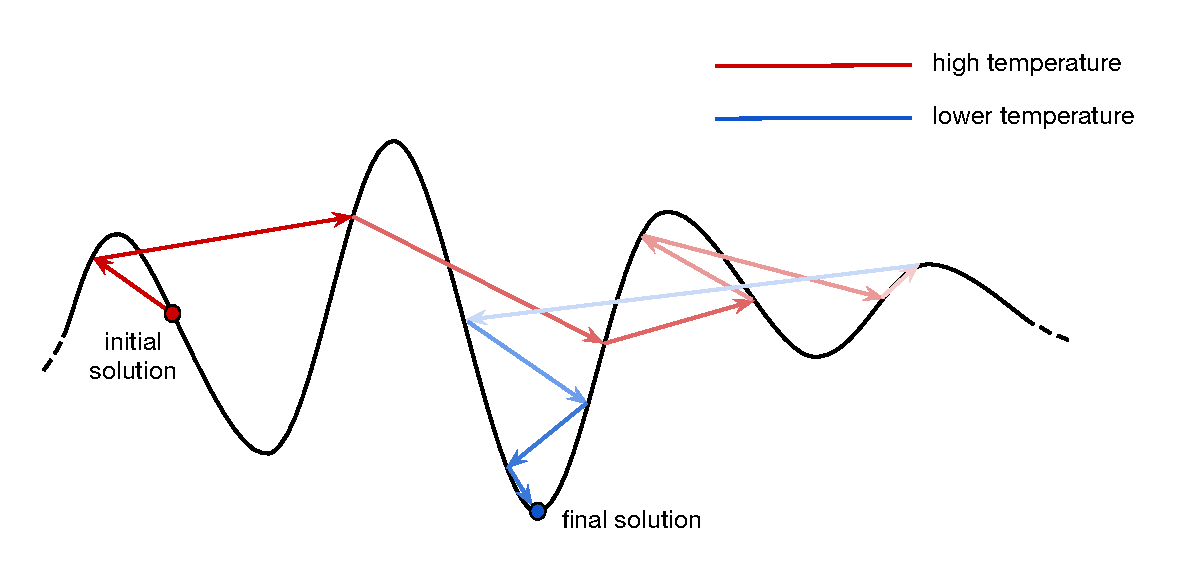
\includegraphics[scale=0.77]{media/sim_annealing.pdf} \\
	\caption{Example of the work of the simulated annealing. Note the initial random exploration with high temperature and the move toward the minima with a lower temperature.}
\end{figure}

\begin{algorithm}
	\caption{Simulated Annealing}\label{Annealing method}
	\hspace*{\algorithmicindent} \textbf{Input:} Admissible solution S \\
	\hspace*{\algorithmicindent} \textbf{Output:} Best solution found
    \begin{algorithmic}[1]
    		\State \textit{let p be the probability to accept a bad move}
    		\State \textit{let T be the temperature}
		\While{! termination condition}
			\State $\Delta \leftarrow$ random 2-OPT move
			\If{$\Delta > 0$}
				\State S $\leftarrow$ perform the move
			\Else 
				\State p $\leftarrow$ f$($T$)$
				\State r $\leftarrow$ random number $\in [0, 1)$
				\If{r $<$ p}
					\State S $\leftarrow$ perform the move
				\EndIf 
			\EndIf
			\If{temperature change condition}
				\State decrease T
			\EndIf
		\EndWhile
		\State \textbf{return} S
    \end{algorithmic}
\end{algorithm}

\noindent Of course the choose of the cooling schedule and the function that regulate the probability to accept a move with respect to the temperature are pivotal and can have a big impact on the performance of the algorithm itself. \\
On our implementation we followed the procedure showed in the paper \cite{simAn} that we are going to briefly explain.
Let X be the initial solution and Y a solution produced after a random 2-OPT move on x, let $f(X)$, $f(Y)$ be the cost respectively of X and Y, let $p_0$ be the initial probability. On each iteration, until the temperature list is full, generate a new Y. If $f(Y) > f(X)$ (pejorative move) compute a temperature with the following formula:
\begin{equation*}
t = \frac{-\vert f(y) - f(x) \vert}{\ln{(p_0)}}
\end{equation*}
otherwise, if $f(Y) < f(X)$, put X = Y and then compute t in the same way.
Now to describe the remaining part of our implementation let's consider N, that is a parameter decided by the user that indicate the maximum number of iteration where we use the same temperature. Let also i = 0, 1... N be a counter for those iteration. We start by extracting $T_{max}$ from the temperature list, this will be the temperature of the system for the next following N iteration. On each iteration we generate a random 2-OPT move: if it is meliorative the solution is simply updated. If it is pejorative we compute a probability $p_i$ defined as:
\begin{equation*}
p_i = \exp \Bigl( \frac{-(f(Y)-f(X))}{t_{max}} \Bigr)
\end{equation*}
then we generate a random number $r_i \in [0, 1)$ and if $r_i < p_i$ the move is accepted.
At this point, if we accept a bad move, we need to calculate another temperature $T_i$, defined as:
\begin{equation*}
T_i = \frac{-d_i}{p_i}
\end{equation*} 
where $d_i$ is the difference between $f(Y)$ and $f(X)$ on iteration i. We need also to keep in memory a counter c for each time we have performed a pejorative move. When we reach N iteration, we have to decrease the temperature: we compute the mean
\begin{equation*}
T_{mean} = \frac{1}{c} \sum T_i
\end{equation*}
and we substitute $T_{max}$ with $T_{mean}$. Since $T_i < T_{max}$ we have also that $T_{mean} < T_{max}$ so with the substitution we decrease the temperature. Now we pick another $T_{max}$ and we repeat the entire procedure until the algorithm terminate.



\subsection{Genetic Algorithm}
The genetic algorithm is inspired by the evolution theory, formulated by Charles Darwin during the $18^{th}$ century. 
The algorithm starts with a population where each individual that belong to the population itself is a solution to the problem, so in our case each individual is a solution for the TSP. Each individual has also a fitness that is defined as the cost of the solution. On each iteration (also called epoch), the individuals that have the highest fitness are removed from the population: maintaining the parallelism with the evolution theory we can say that the individuals that didn't adapt to the environment (high fitness) died.
On each iteration we have also that couples of individuals reproduce and the new elements substitute the ones that we have removed (so the population size remain constant). The children generated inherit characteristics from both their parents: a simple mechanism is just to pick part of the edges from one parent and the remaining from the other. Of course in this way the children is not a solution of the TSP problem cause some node may be visited more than once or may miss, so a repair function is required. In addition, at this point, a mutation function can be added: this mean that a children with probability x (that in general is low) can suffer a modify that hasn't any relation with its parents, like a random exchange of two vertices in the visit sequence. We can introduce this shrewdness to emulate in the algorithm the mutation mechanism that happens also in real life\\
After some iteration we have that the average fitness improve due to the fact that we remove bad solution and we generate new solution from the better ones. When the algorithm end, the champion of the population, that is the solution with the best fitness, is the final result. \\


\begin{algorithm}
	\caption{Genetic}\label{Genetic method}
	\hspace*{\algorithmicindent} \textbf{Input:} Population $P_t$ of solutions S, N number of new element per epoch \\
	\hspace*{\algorithmicindent} \textbf{Output:} Best individual of the population
    \begin{algorithmic}[1]
    		\State $\textit{t} \leftarrow 0$
    		\State $\textit{bestSolution}$
    		\State $\textit{fitnessList}$
    		\State fitnessList, bestSolution $\leftarrow$ computeFitness$(P_t)$ 
    		\While{! condition of termination}
    			\For{i $=$ 0, i $<$ N, i++}
    				\State removeElement$(P_t)$
    				\State update$($fitnessList$)$
    			\EndFor
    			\For{i $=$ 0, i $<$ N, i++}
    				\State S $\leftarrow$ generateNewChildren$(P_t)$
    				\State repair$($S$)$
    				\State fitnessList $\leftarrow$ add$($fitness$($S$))$
    				\If{fitness$($S$) < $ fitness$($bestSolution$)$}
    					\State bestSolution $\leftarrow S$
    				\EndIf
    			\EndFor
    			\State \textit{t} $\leftarrow$ t+1
    		\EndWhile
    		\State \textbf{return} bestSolution 
    \end{algorithmic}
\end{algorithm}


\noindent Our first implementation of this algorithm was pretty simple. We generated a population of a size decided by the user using the GRASP algorithm. We created a probability mass function (PMF) normalizing the sum of the fitness, so on each iteration we randomly chose the elements to remove based on that mass function. This means that during the firsts iterations, when all the individual have almost the same fitness, the element are almost randomly remove, while when the algorithm progress and there is a more evident difference between good and bad individuals, with high probability only the worst solutions are removed. The number of element to remove on each iteration (that is equal to the number of children to generate) is a parameter decided by the user. \\
To reproduce two elements we used the following technique: we chose a random number x between 0.3 and 0.7. Then we picked the first x visited node from one of the parent and the remaining from the other. At this point we used a repair function (Figure \ref{fig:genetic}) that remove all the points visited twice and insert the missing ones using the insertion algorithm described in 5.1.3. 

\begin{figure}[h!]
  \centering
  \begin{subfigure}[b]{0.49\linewidth}
    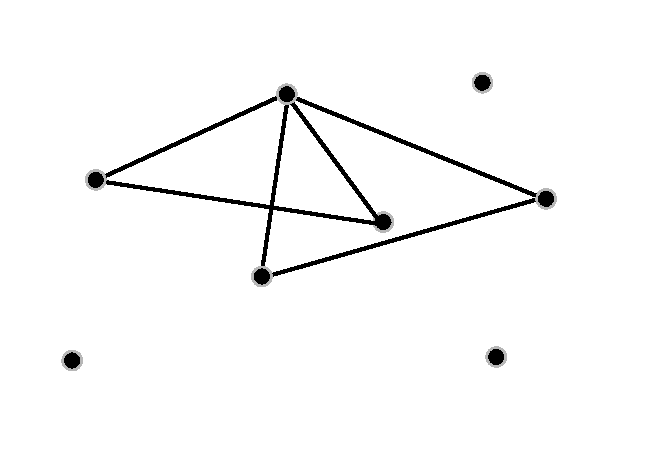
\includegraphics[width=\linewidth]{media/gene1.pdf}
     \caption{Non repaired children}
  \end{subfigure}
  \begin{subfigure}[b]{0.49\linewidth}
    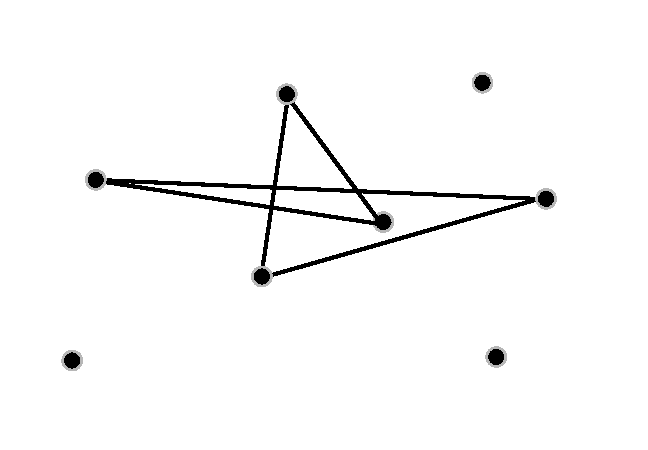
\includegraphics[width=\linewidth]{media/gene2.pdf}
    \caption{Twice-visited vertices removal}
  \end{subfigure}
  \begin{subfigure}[b]{0.49\linewidth}
    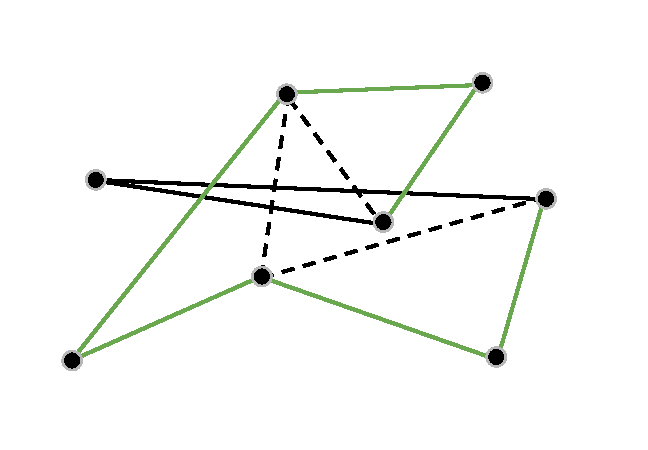
\includegraphics[width=\linewidth]{media/gene3.pdf}
    \caption{Insertion of remaining element}
  \end{subfigure}
  \begin{subfigure}[b]{0.49\linewidth}
    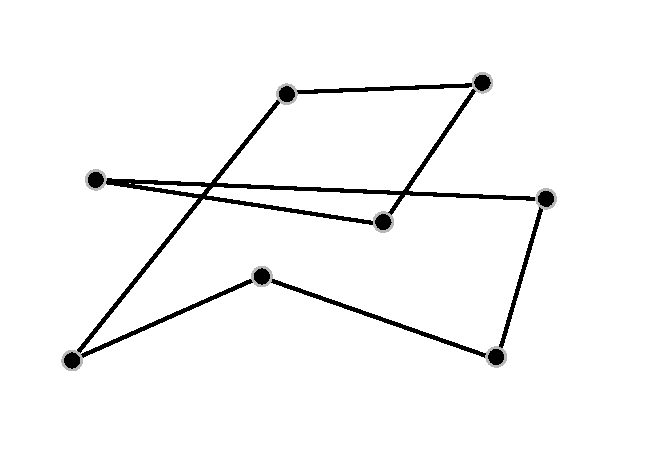
\includegraphics[width=\linewidth]{media/gene4.pdf}
    \caption{Final result}
  \end{subfigure}
  \caption{Example of the steps of a repair function}
  \label{fig:genetic}
\end{figure}

\noindent The couples to reproduce are simply chosen at random from the population and we didn't implement any mechanism to control that same individual aren't choose more than once. We made this choice because on this algorithm the population have often big size, in general more than 10000 individuals, so the probability to pick the exactly same individuals more than once is very low.
After some run, plotting the average fitness and the best fitness, we could observe the 
expected behaviour (Figure \ref{fig:fitness}): the average fitness continuously decrease until it get closer to the best fitness (that improve only sometimes).  \\

\begin{figure}[h!]
\centering
	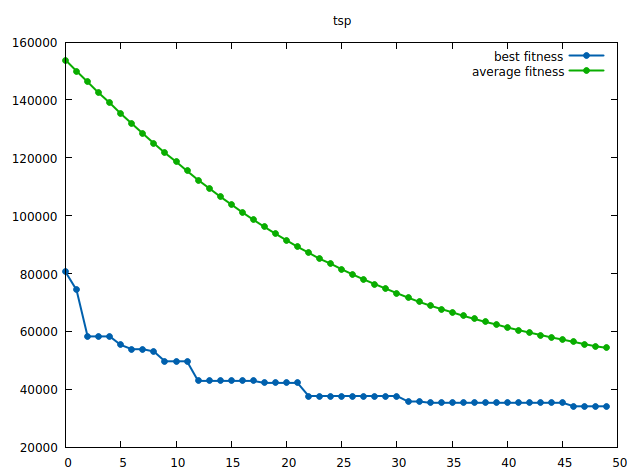
\includegraphics[scale=0.6]{media/fitnessPlot.png} \\
	\caption{Plot of the average fitness and best fitness during the execution of a genetic algorithm.}
	\label{fig:fitness}
\end{figure}

\noindent The problem of our implementation became evident after testing it on different instances: the solutions had lot of intersection (like the ones generated by the GRASP algorithm) that of course don't belong to the optimum. An example of this can be seen on Figure \ref{fig:geneticplot}. So we tried to introduce the 2-OPT someway inside the genetic. From this point, to distinguish the different versions of the genetic that we realized, we will call the implementation just described \textit{genetic 1}. \\
A possibility that we first considered but we immediately discarded was to just apply the 2-OPT algorithm on the final solution provided by the genetic. This didn't make lot of sense because we did a lot of effort to produce a result with the genetic and then we discard a consistent part of it using the 2-OPT: a simple GRASP plus 2-OPT would be more efficient.
Then we decided to add the 2-OPT to the repair function. So each children, after being repaired was also refined using the 2-OPT rule. Let's call this version \textit{genetic 2}. We immediately noticed a large reduction of the number of epochs executed in the same amount of time with respect to genetic 1. This is because the populations used in the genetic algorithm are large and even if 2-OPT is quite fast it has to be executed a lot of time. \\
Finally we tried an hybrid approach between genetic 1 and genetic 2: after the repair function the refinement is executed with a probability x decided by the user. With this version each epoch is faster than genetic 2 because the 2-OPT is executed less time, however the price of this is the introduction of another parameter that is the probability x.\\

\begin{figure}[h!]
\centering
	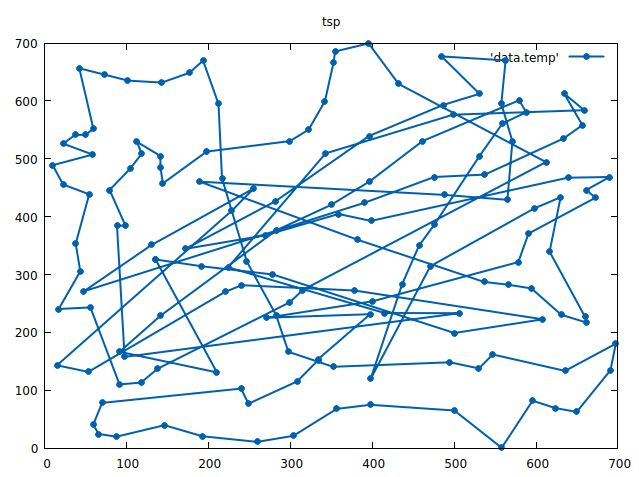
\includegraphics[scale=0.6]{media/genetic.png} \\
	\caption{Solution of the instance ch150 provided by our first implementation of the genetic. Note the big number of edge intersections.}
	\label{fig:geneticplot}
\end{figure}

\noindent We tested these three versions on the dataset to find which ones is the best. We establish a time limit of 10 minutes and a population size of 2000 elements with 200 new elements each epoch. The 2-OPT, when applied inside the repair function, has a time limit of one second. Note that we were forced to use a population with a limited size, in fact after few tests we discovered that it's very difficult to handle a big population (like 10000 or more elements) on a single machine, cause the algorithm became incredibly slow.
The Table \ref{tab:meta} report the final values of the objective functions obtained by each algorithm and the number of epoch that it was able to execute within the time limit. The first thing that we can notice, as expected, is that the introduction of the 2-OPT involves a big decrease of the epochs performed. However in both genetic 2 and 3 results are better, so even if we pay an increase of execution time for each epoch, the addition of the refinement is worth. This became more evident if we consider the performance profile (Figure \ref{fig:geneticPP}), where genetic 1 is far the worst algorithm. \\ 
Again, looking to the performance profile, genetic 2 seems to be the best, followed by genetic 3 that is slightly worse. However we chose genetic 3 as the winner of this first ``eliminatory phase" for the following reasons: first of all the difference in the performance profile is tiny and since the dataset used is quite small we cannot say with absolute certainty that genetic 2 is the best. Moreover if we perform a 2-OPT on each new element, we move away from the idea of the genetic, in fact each children has to pass through a repair function and then a refinement, so with high probability it will maintain very few elements of its parents. Finally we execute very few epochs with respect to genetic 1 and 3 and this is against the principle of the evolution of the population. So this is why we selected the third version of the algorithm to compete with the others metaheuristics.\\

\begin{table}[h!]
	\begin{center}
		\begin{tabular}{l|c|c|c|c|c|c}
			\textbf{Instance} & \textbf{Genetic 1} & \textbf{Epochs} & \textbf{Genetic 2} & \textbf{Epochs} & \textbf{Genetic 3} & \textbf{Epochs}\\
			& & & & & & \\
			\hline
			d657 & 58281 & 67 & 51628 & 6 & 51485 & 13 \\
			d1291 & 82270 & 9 & 60116 & 2 & 61857 & 3 \\
			fl417 & 13066 & 247 & 12040 & 3 & 12046 & 6 \\
			fl1400 & 29775 & 8 & 21836 & 2 & 21635 & 3 \\
			fl1577 & 37798 & 6 & 27996 & 1 & 30190 & 2 \\
			nrw1379 & 77437 & 7 & 65374 & 2 & 67865 & 3 \\
			p654 & 39289 & 67 & 34986 & 2 & 35216 & 5 \\
			pcb1173 & 83380 & 12 & 63693 & 2 & 63075 & 3 \\
			pcb3038 & 224091 & 1 & 217479 & 0 & 220982 & 0 \\
			pr1002 & 342579 & 19 & 278606 & 2 & 278935 & 4 \\
			pr2392 & 635460 & 1 & 566707 & 0 & 576564 & 0 \\
			rl1304 & 396680 & 9 & 316148 & 2 & 315956 & 3 \\
			rl1323 & 430922 & 8 & 325125 & 2 & 341412 & 3 \\
			rl1889 & 532907 & 3 & 486805 & 1 & 490274 & 1 \\
			u724 & 50800 & 48 & 44697 & 3 & 44857 & 7 \\
			u1060 & 309589 & 17 & 240649 & 2 & 241563 & 4 \\
			u2152 & 111343 & 1 & 98474 & 0 & 99573 & 0 \\
			u2319 & 316450 & 1 & 295777 & 0 & 297665 & 0 \\
			vm1084 & 326657 & 15 & 255282 & 2 & 258157 & 4 \\
			vm1748 & 502384 & 3 & 460075 & 1 & 480036 & 1 \\
		\end{tabular}
		\caption{Results of the eliminatory between the different versions of the genetic we implemented}
		\label{tab:meta}
	\end{center}
\end{table}

\begin{figure}[h!]
\centering
	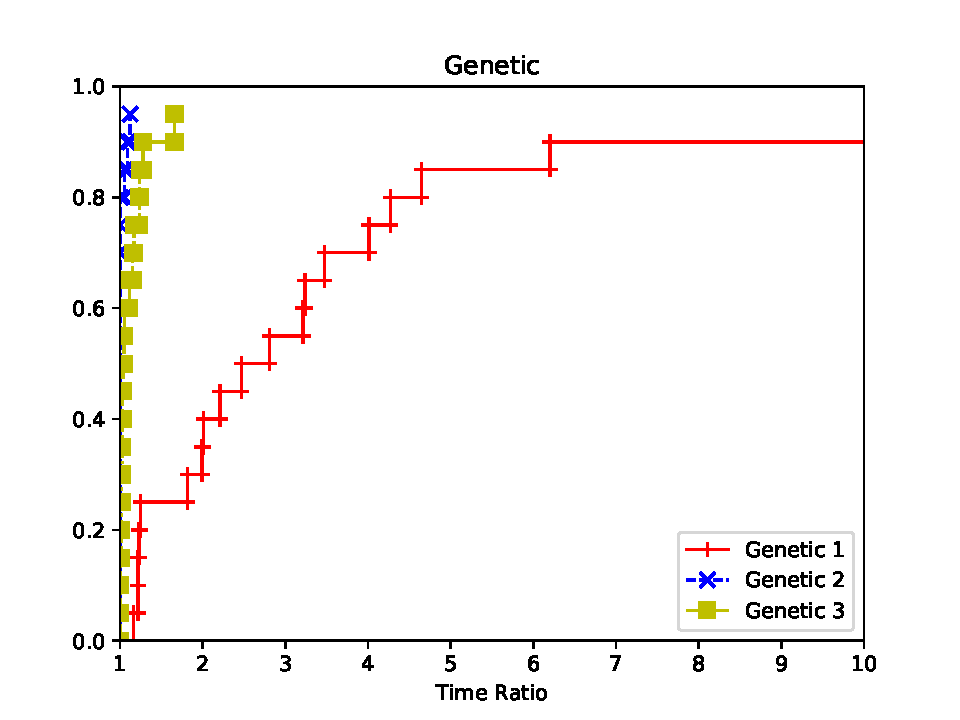
\includegraphics[scale=0.9]{media/genetic.pdf} \\
	\caption{Performance profile of the three versions of the genetic algorithm we implemented}
	\label{fig:geneticPP}
\end{figure}

\noindent To conclude we noticed that the genetic algorithm is well suited to a distributed approach. On the big data domain, when, for example, we need to perform a clustering algorithm, a possible solution is to split the set of points into smaller chunks, and locate them on different machines that execute the operations on them independently. We can think to a similar solution for the genetic: we can divide a big population into smaller subset, assign each of them to a different machine (or a different core if we have only one computer) and apply the algorithm. Considering the parallelism with the evolution theory, we can think to this as if we have different populations living in different habitats. At this point it is also possible to introduce ``migrations" between different populations, this means that on each epoch we can randomly shuffle some elements between different subsets. 
So with this strategy we can run the genetic on a cluster, solving the problem of having to menage a big population and speeding up the execution of the algorithm.


\subsection{Final comparison between metaheuristics}

\begin{figure}[h!]
\centering
	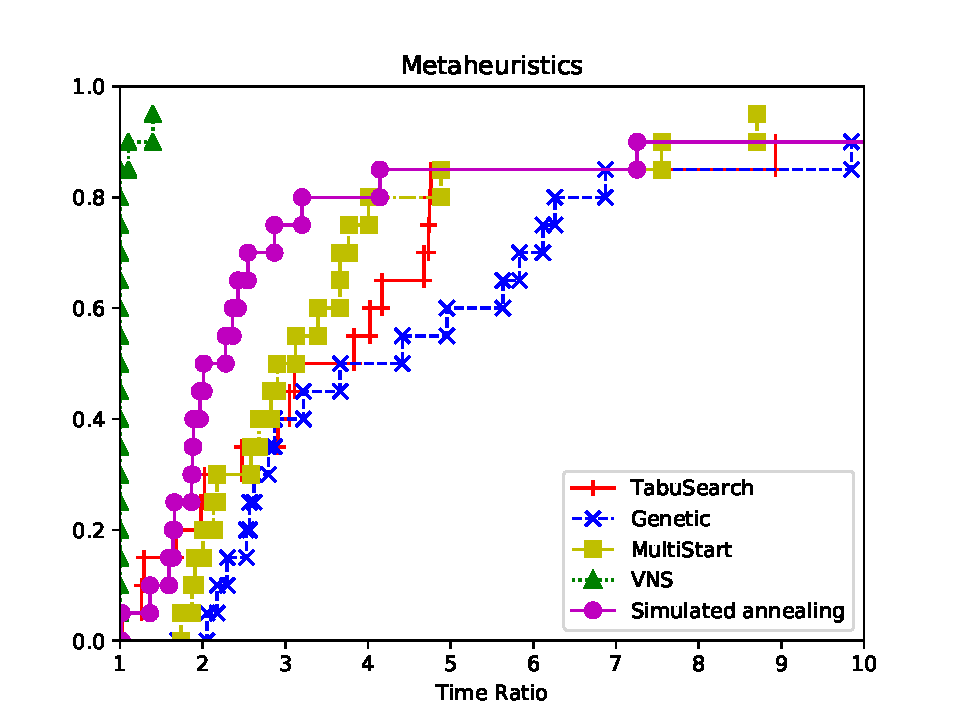
\includegraphics[scale=0.9]{media/metaheuristics.pdf} \\
	\caption{Performance profile of the metaheuristics}
	\label{fig:metaheuristics}
\end{figure}

On Figure \ref{fig:metaheuristics} it is possible to see the performance profile of all the metaheuristics we analyzed in this section. We tested each algorithm on the usual dataset with a time limit of 30 minute per instance (all the other details about the experiments are report on section \ref{euristic_num_res}). The parameter we used are the following:

\begin{itemize}
	\item \textbf{Multi start}: no parameter except for time limit.
	\item \textbf{VNS}: 5-OPT random move for the kick.
	\item \textbf{Tabu search}: tenure equals to 40\% of the instance size.
	\item \textbf{Simulated annealing}: temperature list of 5000 elements, 1000 iteration with the same temperature.
	\item \textbf{Genetic}: population size of 2000, 200 new elements per epoch. 
\end{itemize}

\noindent The first thing we can notice is that the VNS has the best performance. Of course our dataset is quite small, so we cannot say with absolute certainty that VNS is in absolute the best algorithm. However our results are aligned with the ones we saw during the course and the ones obtained by other students, so we can conclude that VNS is a very good heuristic solution for the TSP. \\
Another thing we can notice are the poor performance of the genetic. This result was expected due to the fact we were forced to use small populations and to introduce the 2-OPT at the expense of the number of epoch for each run. \\
Finally, noteworthy is the simulates annealing that seems to have very good performance.
